\begin{titlepage}
	
	\hspace{-0.6in}{
		\begin{picture}(0,0)
		{
				
\includegraphics{img/Title_MSE.png}
		}
		\end{picture}
	}
	
	\begin{flushright}
	\begin{picture}(144,0)
	{
			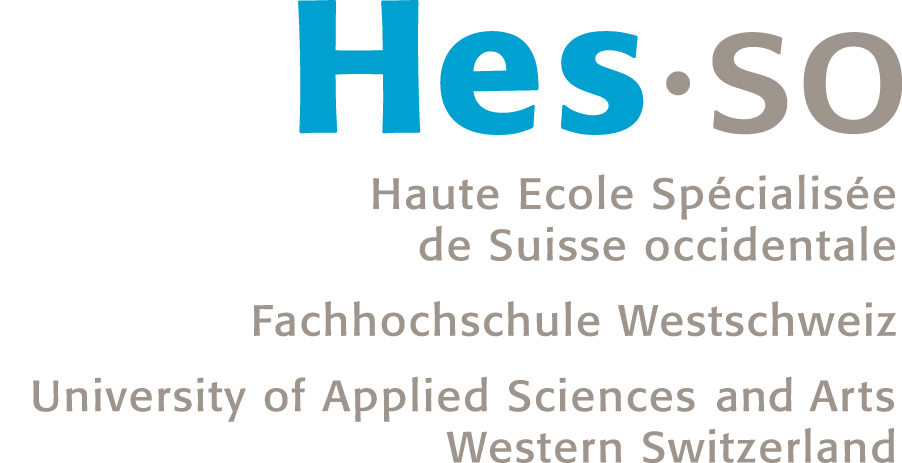
\includegraphics[width=50mm]{img/Title_Hesso.png}
	}
	\end{picture}
	\end{flushright}
	
	\begin{flushleft}
		\hspace{-0.6in}{
			\parbox{10cm}{
				\small
				Master of Science HES-SO in Engineering\\
				Av. de Provence 6\\
				CH-1007 Lausanne\\
			}
		}
	\end{flushleft}
	
	\begin{center}
	\large
	\textsc{\MakeUppercase {}}\\
	\end{center}
	
	
	\begin{flushright}
		\vspace*{1cm}
		\huge
		Master of Science HES-SO in Engineering\\
		
		\vspace{0.5cm}
		\large
		Orientation: Technologies de l'information et de la communication (TIC)\\
		\vspace*{1cm}
		\huge
		\MakeUppercase {Serious Game 3D temps réel}
		
		\MakeUppercase{pour la réhabilitation}\\
		
		\normalsize
		\vspace{4.5cm}
		Fait par\\
		\huge
		Nicolas Wenk\\
		
		\vspace{1cm}
		\normalsize
		Sous la direction de\\
		Prof. Nabil Ouerhani\\
		Dans le groupe de compétence Imagerie de la HE-Arc\\
		
		\vspace{1cm}
		Expert externe: Quentin Silvestre
		
		\vspace{1cm}
		Lieu, HES-SO//Master, 2016\\
		
	\end{flushright}

\end{titlepage}
